%% March 2018
%%%%%%%%%%%%%%%%%%%%%%%%%%%%%%%%%%%%%%%%%%%%%%%%%%%%%%%%%%%%%%%%%%%%%%%%%%%%
% AGUJournalTemplate.tex: this template file is for articles formatted with LaTeX
%
% This file includes commands and instructions
% given in the order necessary to produce a final output that will
% satisfy AGU requirements, including customized APA reference formatting.
%
% You may copy this file and give it your
% article name, and enter your text.
%
%
% Step 1: Set the \documentclass
%
% There are two options for article format:
%
% PLEASE USE THE DRAFT OPTION TO SUBMIT YOUR PAPERS.
% The draft option produces double spaced output.
%

%% To submit your paper:
\documentclass[draft,linenumbers]{agujournal2018}
\usepackage{apacite}
\usepackage{url} %this package should fix any errors with URLs in refs.
%%%%%%%
% As of 2018 we recommend use of the TrackChanges package to mark revisions.
% The trackchanges package adds five new LaTeX commands:
%
%  \note[editor]{The note}
%  \annote[editor]{Text to annotate}{The note}
%  \add[editor]{Text to add}
%  \remove[editor]{Text to remove}
%  \change[editor]{Text to remove}{Text to add}
%
% complete documentation is here: http://trackchanges.sourceforge.net/
%%%%%%%


%% Enter journal name below.
%% Choose from this list of Journals:
%
% JGR: Atmospheres
% JGR: Biogeosciences
% JGR: Earth Surface
% JGR: Oceans
% JGR: Planets
% JGR: Solid Earth
% JGR: Space Physics
% Global Biogeochemical Cycles
% Geophysical Research Letters
% Paleoceanography and Paleoclimatology
% Radio Science
% Reviews of Geophysics
% Tectonics
% Space Weather
% Water Resources Research
% Geochemistry, Geophysics, Geosystems
% Journal of Advances in Modeling Earth Systems (JAMES)
% Earth's Future
% Earth and Space Science
% Geohealth
%
% ie, \journalname{Water Resources Research}

\journalname{Water Resources Research}

\usepackage{booktabs}
\usepackage{longtable}
\usepackage{array}
\usepackage{multirow}
\usepackage{wrapfig}
\usepackage{float}
\usepackage{colortbl}
\usepackage{pdflscape}
\usepackage{tabu}
\usepackage{threeparttable}
\usepackage{threeparttablex}
\usepackage[normalem]{ulem}
\usepackage{makecell}
\usepackage{xcolor}

\usepackage{soulutf8}

\begin{document}

%% ------------------------------------------------------------------------ %%
%  Title
%
% (A title should be specific, informative, and brief. Use
% abbreviations only if they are defined in the abstract. Titles that
% start with general keywords then specific terms are optimized in
% searches)
%
%% ------------------------------------------------------------------------ %%

% Example: \title{This is a test title}

\title{Development and testing of a new model of the variable connected
fractions of Prairie basins}

%% ------------------------------------------------------------------------ %%
%
%  AUTHORS AND AFFILIATIONS
%
%% ------------------------------------------------------------------------ %%

% Authors are individuals who have significantly contributed to the
% research and preparation of the article. Group authors are allowed, if
% each author in the group is separately identified in an appendix.)

% List authors by first name or initial followed by last name and
% separated by commas. Use \affil{} to number affiliations, and
% \thanks{} for author notes.
% Additional author notes should be indicated with \thanks{} (for
% example, for current addresses).

% Example: \authors{A. B. Author\affil{1}\thanks{Current address, Antartica}, B. C. Author\affil{2,3}, and D. E.
% Author\affil{3,4}\thanks{Also funded by Monsanto.}}

\authors{
Kevin Shook
\affil{1}
\thanks{Kevins thanks}
John Pomeroy
\affil{1}
\thanks{Current address: Some other place, Germany}
Kevin Shook
\affil{1, 2}
}


% \affiliation{1}{First Affiliation}
% \affiliation{2}{Second Affiliation}
% \affiliation{3}{Third Affiliation}
% \affiliation{4}{Fourth Affiliation}

\affiliation{1}{Centre for Hydrology, University of Saskatchewan}
\affiliation{2}{Global Water Futures, University of Saskatchewan}
%(repeat as many times as is necessary)

%% Corresponding Author:
% Corresponding author mailing address and e-mail address:

% (include name and email addresses of the corresponding author.  More
% than one corresponding author is allowed in this LaTeX file and for
% publication; but only one corresponding author is allowed in our
% editorial system.)

% Example: \correspondingauthor{First and Last Name}{email@address.edu}
\correspondingauthor{Kevin Shook}{Kevin.Shook@usask.ca}

%% Keypoints, final entry on title page.

%  List up to three key points (at least one is required)
%  Key Points summarize the main points and conclusions of the article
%  Each must be 100 characters or less with no special characters or punctuation

% Example:
% \begin{keypoints}
% \item	List up to three key points (at least one is required)
% \item	Key Points summarize the main points and conclusions of the article
% \item	Each must be 100 characters or less with no special characters or punctuation
% \end{keypoints}

\begin{keypoints}
\item List up to three key points (at least one is required)
\item Key Points summarize the main points and conclusions of the article
\item Each must be 100 characters or less with no special characters or
punctuation
\end{keypoints}

%% ------------------------------------------------------------------------ %%
%
%  ABSTRACT
%
% A good abstract will begin with a short description of the problem
% being addressed, briefly describe the new data or analyses, then
% briefly states the main conclusion(s) and how they are supported and
% uncertainties.
%% ------------------------------------------------------------------------ %%

%% \begin{abstract} starts the second page

\begin{abstract}
TBD
\end{abstract}
\section{Introduction}

It has been known for more than 60 years
\citep{stichlingDRAINAGEAREAHYDROLOGIC1957} that the regions within
Canadian Prairie basins which can contribute flow to their outlet are
temporally and spatially variable. The cause of the variability is the
unusual hydrography of the Prairies, which was formed by glacial and
post-glacial processes. As the region is semi-arid, and flat, and
deglaciation ocurred \textasciitilde{}10,000-12,000 years B.P.
\citep{christiansenWisconsinanDeglaciationSouthern1979}, there has not
been sufficient water, energy, or time for conventional drainage
networks to form. Consequently, there are few streams within the region.
The largest rivers in the region (the Saskatchewan and its tributaries)
are sourced from the Rocky Mountains and their foothills.

In the absence of streams, much of the region is dominated by the
presence of millions of depressions, known locally as ``sloughs'' or
``potholes''. The depressions trap water from direct precipitation, the
trapping of blowing snow, and can recieve surface runoff. Because much
of the region is underlain by deep deposits of glacial till, which is
largely impermeable, there is generally little interaction between the
depressions and groundwater, although very shalllow interchanges can
occur. In the absence of artificial drainage, most of the losses of
water from the depressions are due to evaportation and
evapotranspiration from the surrounding vegetation.

Many attempts have been made to model the variability using a variety of
models. All of the models developed to date have had limitations which
have restricted their general application within the region. The
methodology of \citep{shawTopographicAnalysisPrairie2012} was restricted
to a single basin. As the relationships controlling the connected
fraction were not quantified, it could not be applied to other
locations. \citet{shookMemoryEffectsDepressional2011} and
\citet{shookStorageDynamicsSimulations2013} developed 2 models for
simulating the connected fractions of Prairie basins. The Wetland DEM
Ponding Model (WDPM) applies simulated fluxes of water (precipitation,
runoff, evaporation, infiltration) to a digitial elevation model (DEM).
Using the algorithm of \citet{shapiroMAPCALCAlgebraGIS1992}, the applied
water is redistributed over the DEM, ponding in depressionsm, and
draining from the basin's outlet. Although the spatial distributions of
water produced by the program appeared to agree well with remotely-
sensed data
\citep{armstrongUSINGWETLANDPONDING2013a, shookStorageDynamicsSimulations2013},
the WDPM was too slow to be used as a component of a hydrological model.

\citet{shookMemoryEffectsDepressional2011} and
\citet{shookStorageDynamicsSimulations2013} developed the Pothole
Cascade Model (PCM) which used discrete ponds, similar to the model of
\citet{shawInfluenceContributingArea2009}, to simulate the variable
connected fractions of Prairie basins. When parameterised with pond
sizes and distribtutions for a given basin, PCM produced very similar
connected-fractions to those estimated by the WDPM for the same location
\citep{shookStorageDynamicsSimulations2013}. Both models demonstrated
very strongly hysteretic relationships between the connected fraction
and the depressional storage of a basin. The hysteresis was demonstrated
to be caused by the disconnection of all depressions as soon as
subtractive fluxes were applied, and to the very differing effects of
additive and subtractive fluxes on the frequency distributions of pond
areas \citep{shookStorageDynamicsSimulations2013}. Hysteresis was
demonstrated to be a feature of the response of depression-dominated
hydrological basins, occurring between the upland runoff and consequent
inflows to a given depression
\citep{shookTransformationFrequencyDistributions2015}.

The PCM algorithm was added to the Cold Regions Hydrological Modelling
(CRHM) platform, which is a physically-based model capable of simulating
Prairie hydrological processes
\citep{pomeroyColdRegionsHydrological2007d}. The addition of the PCM was
shown to dramatically improve the modelled hydrological responses of a
Prairie basin \citep{pomeroyImprovingTestingPrairie2014}. However, as
was demonstrated by \citet{shookMemoryEffectsDepressional2011}, the
simulated connected fraction produced by the PCM depends on the number
of simulated depressions used. When few depressions are used in a
simulations, they do not well represent the shape of the
connected-fraction curve of a basin with many depressions.
Unfortunately, it is difficult to incorporate the very large numbers of
depressions found in a Prairie basin in a hydrological model. Each
depression has several parameters (area, depth, volume, shape) which add
to the complexity of the model. Worse, the connectivity of each
depression must also be determined, which is an onerous task. In the
case of \citet{pomeroyImprovingTestingPrairie2014}, 46 depressions were
used for each sub-basin modelled, which was too few to give a good
representation, but was about all that could be managed by the model.
The outflows from the small number of simulated depressions were
upscaled to represent the outflows from the sub-basin.

\citet{mekonnenImprovedLandSurface2014} developed PDMROF, which is a
very simple representation of the connected fraction of a Prairie basin,
and which can be easily incorporated in any hydrological model. PDMROF
is based on the PDM model of \citet{moorePDMRainfallrunoffModel2007a}.
PDMROF is based on the assumptions:

\begin{enumerate}
\item
  that the volumes of depressions can be represented as a power-law
  distribution
\item
  that the depressions are filled in order from smallest to largest, and
  that the contributing fraction can therefore be estimated by
  integrating the power-law volume distribution, based on the volume of
  storage within the basin.
\item
  that the contributing fraction decreases due to water removal in the
  same manner as which it increases.
\end{enumerate}

There are several problems with this approach.

Researchers have indeed demonstrated that the areas of Prairie ponds,
and therefore of the depressions which contain them \emph{approximate}
power-law distributions, although it has been demonstrated that they are
better approximated by Pareto II distributions {[}{]}. The relationship
between the volume and area of a single depression was shown by
\citep{hayashiSimpleEquationsRepresent2000} to approximate that of a
paraboloid. Therefore the frequency distrbution of the volumes of
depressions is not the same as that of the areas.

The assumption that depressions are filled in the order of their sizes
has several flaws. The first is that it ignores the role of gatekeeping
in controlling flows. The second flaw lies with the implementation of
the filling. As explained by \citet{mekonnenImprovedLandSurface2014},
runoff generated within a landscape unit is assigned to the integrated
storage volume. The fraction of the storage volume which is filled then
generates runoff, the rest of the runoff filling up the remaining
storage. The problem with this methodology is that it ignores the actual
mechanisms by which depressions fill. As described above, Prairie
depressions are filled through a) direct precipitation, b) trapping of
blowing snow and c) through runoff. All three of these mechanisms have
very different contributing areas. As was shown by
\citet{shookStorageDynamicsSimulations2013}, the relationship between
the basins contributing runoff directly to a Prairie depression, and the
areas of depressions, can be described by power-laws, with exponents
smaller than 1.0. Therefore the relative area draining to a depression
decreases with increasing depressional area. Not only does the PDMROF
filling use the incorrect runoff area, it cannot properly calculate the
contributing fraction of a basin.

The third assumption is evidenly incorrect. When a set of filled
depressions is subjected to subtractive fluxes (evaporation,
infiltration) they all become unfilled. Thus their individual, and
collective, connected fractions are instantly zero. As water is
progressively removed, ponds will shrink, disconnect and disappear.
Therefore, as was found by \citet{shookMemoryEffectsDepressional2011}
and \citet{shookStorageDynamicsSimulations2013}, the size distributions
of pond areas change very differently when adding and removing water.
The processes are not reversible, so there is no way that the connected
fraction curves can be of the same shape.

Nevertheless, PDMROF has been shown to do a good job in simulating the
contributing fraction of a small Prairie basin in a hydrological model
\citep{mengistuTestingAbilitySemidistributed2016}. It is noticable that
it was necessary to calibrate the model parameters, unlike those of PCM.
The requirement for calibration is related to the deficiencies of PDMROF
noted above - were the model based on better assumptions, its parameters
might be set from remote sensing/GIS.

Figure 2 plots the filling and emptying curves computed using WDPM for
the St.~Denis sub-basin above pond 90. The curves computed by PDMROF,
using parameters determined by
\citet{mengistuTestingAbilitySemidistributed2016} are also plotted. It
is noticeable that the PDMROF curves are quite similar the WDPM filling
curve. \citet{mengistuTestingAbilitySemidistributed2016} reported that
in all of their simulations the contributing fraction of the basin was
smaller than 0.35. In this region, PDMROF splits the difference between
the rising and falling limbs of the WDPM curves. Had the volumetric
storage been greater, there would likely have been greater discrepencies
between the two models.

\begin{figure}[h]
\includegraphics[width=1\linewidth,]{figures/SD_above_90_WDPM_PDMROF} \caption{Connected/contributing fractions vs. fractional volume for WDPM and PDMROF, for St. Denis Basin above Pond 90.}\label{fig:unnamed-chunk-2}
\end{figure}

The need to calibrate PDMROF is also its great weakness. In the Canadian
Prairies, there are few stream gauges, and consequently stream basins
are very large. Of the 217 currently active stream gauging stations
within the Canadian Prairies, the median gross basin area is 573
km\textsuperscript{2} (mean = 1238 km\textsuperscript{2}). Therefore,
any stream basin modelled in the Prairies will have very large regions
which are combined together for calibrating the PDMROF parameters. No
matter how well the model is distributed for its forcings, and state
variables, the hydraulic parameters will always be lumped at the scale
of the basin.

The implications of the lumping are demonstrated by the behaviour of the
full St.~Denis basin. The full basin is dominated by the presence of a
large pond near the outlet. In fact, the basin does not have a
traditional outlet, as it has no permanent stream. The outlet is simply
the lowest point on the basin divide - much of the basin lies below the
outlet. Therefore St.~Denis basin is endorheic, and has never been known
to spill in the period of monitoring. As demonstrated in , the
connected-fraction curve for St.~Denis basin is completely different
from that of the sub-basin above pond 90. Note that as there have never
been any flows recorded from the outlet, it would be impossible to
calibrate PDMROF for the basin. Therefore, it is not a good practice to
use a calibrated PDMROF relationship for any other basin, even when it
lies entirely within the same landform and land use type. As Prairie
basins are very large, the use of calibrated models like PDMROF will
invariably lump together many different regions, with very different
contributing fractions, resulting in poor simulations.

\subsection{Research objectives}

The overall objective of this research is to develop and test a new
method for simulating the variable conencted/contributing fractions of
Prairie basins. The method is to have the following characteristics

\begin{enumerate}
\item
  It must be generic, able to estimate the connected/contributing
  fraction for any Prairie basin.
\item
  It must be able to simulate the hysteretic relationship between the
  connected fraction and the storage of water in a basin.
\item
  It must be able to be parameterized from GIS/remote sensing, without
  use of any form of calibration.
\item
  It must have a reasonably small number of parameters and state
  variables.
\item
  It must be able to execute quickly.
\end{enumerate}

The ideal model will therefore have the generic capacity, hystertic
relationships and simple parameterization of WDPM and PCM, as well as
the small numbers of parameters and states and simplicity of PDMROF.

\section{Materials and Methods}

\subsection{Model background}

The development of the new model is based upon the work of ??, which
found the following:

\begin{enumerate}
\item
  When the a basin is small, the sizes, arrangements and locations of
  all of the depressions are important in controlling the conencted
  fraction.
\item
  As the number of depressions is increased (i.e.~when the basin is
  large), the effect of any single depression is reduced.
\item
  When there are large numbers of depressions, whose size distributions
  approximate a Pareto II distribution (with many more small depressions
  than large ones), then the spatial arrangement of the depressions is
  unimportant, as gatekeeping is very small.
\item
  When there are large numbers of depressions, and there is a single
  large depression, or a few large depressions, then the location of the
  large depression(s) within the basin is important.
\end{enumerate}

In the case of a large number of depressions without a dominant
depression, the connected fraction curve is the integrated area of the
depressions and basins, vs.~the integrated volumes. Although this may
seem to be related to PDMROF, the shape of the curve is very different,
because a) it specifically includes the depression basin areas and b)
the depressions are filled by runoff. The shapes of the rising limbs
were found to approximate 1:1 lines.

\subsection{Model concept}

The concept behind the new model is to combine the effects of the large
number of small depressions, and the few large depressions, in a
flexible manner. The guiding assumption is that the model will be used
in basins large enough that the spatial arrangement of the small
depressions is not terribly important. From {[}?{]} this would appear to
be the case when the number of depressions, with areas greater than 25
m\textsuperscript{2}, is at least 1,000.

\subsubsection{Small depressions}

The state of the small depressions is defined by their fractional
depressional storage and connected areas. Figure 3 plots the connected
fraction computed from 10,000 realizations of 1,000 depressions
simulated from the relationships described in {[}{]}. In each
realization, the depressions were filled from their initial state, by
repeated additions of water. In each addition, the water was applied
evenly to the depression, and its basin, assuming a runoff coefficient
of 1. With each addition of water, the connected fraction was computed
based on the assumption of no gatekeeping - each depression is assumed
to be connected directly to a stream channel. The curves in Figure 3a
represent filling the simulated depressions from their being empty. The
curves in Figure 3b were generated by filling all of the depressions,
and remving 100 mm from each. This results in all of the ponds having
surface elevations being below theier basins' outlets, which causes the
connected fraction of the basin to be zero. Of course, all depressions
with maximum depths smaller than 100 mm will have their water depth
reduced to zero. Following the water removal, the simulated depressions
were then filled iterattively as before. The process was repeated for
removals of 200 mm and 300 mm, as plotted in Figure 3c and d.

\begin{figure}[h]
\includegraphics[width=1\linewidth,]{figures/all_filling_curves} \caption{Connected/contributing fractions vs. fractional volume for 10,000 realizations of 1,000 depressions. The realizations are plotted in grey, the median of all realizations is plottted
as the heavy black line. A 1:1 line is plotted in red.}\label{fig:unnamed-chunk-3}
\end{figure}

Although there is some considerable scatter among the curves, the median
curves are slightly sigmoidal, approximating lines. Very similar results
were found by \citet{shookMemoryEffectsDepressional2011} for
applications and removals of water at Smith Creek Research basin using
the WDPM.

It is important to note that {[}{]} demosntrated that the degree of
scatter among realizations of this type is a function of the number of
depressions being simulated. Only 1,000 depressions are used here;
{[}{]} found over 2000 depressions greater than 25 m\textsuperscript{2}
in a Prairie basin of only 11 km\textsuperscript{2}. Therefore, in a
large basin, the degree of scatter, and therefore the degree of
uncertainty in the filling trajectories, is reduced.

The operation of the proposed parametric model of the hystertic
connected fraction is illustrated by the schematic diagram in Figure 4.
The initial state of the modelled basin (its fractional water volume and
connected fraction) is plotted as point a. When water is removed from
depressional storage, either by evaporation or by infiltration, the
connected fraction becomes zero, and the volume is reduced, as shown by
point b. As water is further removed, the connected fraction remains at
zero, and the fractional water is reduced, as is shown by point c. When
water is added, the connected fraction and fractional volume are
increased, along the trajectory from the current state (point c) to the
filled state, i.e. (1,1), resulting in the new state at point d.

\begin{figure}[h]
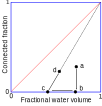
\includegraphics[width=1\linewidth,]{figures/hysteresis_model} \caption{Operation of the parametric hysteresis model of the states of Prairie
basins. The original state is shown at point a. Points b through d show the effects of
removing, then adding water. All states exist below the 1:1 line plotted in red.}\label{fig:unnamed-chunk-4}
\end{figure}

Such a model is very easily implemented. All that is required is to
store the basin's state at each interval. Whenever water is removed, the
connected fraction is set to zero, and the volumetric storage is reduced
as usual. The computation of the connected fraction from the trajectory
to (1,1) only takes a few lines of code. Because the connected fraction
and the volumetric storage are connected, it would be simplest to solve
them iteratively, by dividing the additions of water into very small
depths. Since the Prairies are semi-arid, and hydrological models of the
region are generally run on sub-daily time intervals this is unlikely to
be problematic.

\paragraph{Water areas}

The existing physically-based hydrological models used for the Canadian
Prairies, MESH and CRHM, are based on GRUs and HRUs, respectively.
Incorporation of the parametic hystersis model would result in a single
HRU/GRU being used to represent the water storage. Unfortunately,
neither model currently simulates the relationship between the volume of
water stored in a GRU/HRU and its area, which is important for
calculating the actual evaporation.
\citet{shookMemoryEffectsDepressional2011} showed that the relationship
between the fractional water-covered area and the fractional water
storage is slightly hysteretic.

Figure 5 plots the fractional water cover (fraction of the maximum
possible water-covered area) vs.~the fractional depressional storage for
simulated filling and emptying of a Prairie basin. The blue line plots
the median of the filling curves from an initially-empty basin, the red
line plots the median of the emptying curves, using the 10,000
realizations of 1,000 depressions discussed above. The green line plots
the result that would be expected for a single depression using the
relationship of \citet{hayashiSimpleEquationsRepresent2000}, with an
exponent of 3.33. The purple line plots the same relationship using an
exponent of 1.72. The two values were used by
\citet{pomeroyImprovingTestingPrairie2014} for depressions greater than
or equal to and smaller than 10,000 m\textsuperscript{2}, respectively.
The same values were used for all of the realizations.

\begin{figure}[h]
\includegraphics[width=1\linewidth,]{figures/filling_emptying_water_areas} \caption{Fraction water cover vs. fractional volume for 10,000 realizations of 1,000 depressions. The median rising limb is plotted in blue, the median falling limb is plotted in red. Curves
for a single depression, based on the Hayashi-van der Kamp equations are plotted in green, 
for p = 3.33, and purple for p = 1.72}\label{fig:unnamed-chunk-5}
\end{figure}

The median filling curve lies midaway between the single depression
curves, for values of the fractional depressional storage smaller than
about 0.5, becoming tangent to the p = 3.33 curve. As the depressions
fill roughly in their size order (also affected by their basin areas),
the small ponds are filled first, so the mdeian water area filling curve
will come to resemble that of the large depressions. When the
depressions are emptied, the ponds in small depressions are
progressively elimiated. Thus the emptying curve lies below even the
curve of the single depressions with exponent values of 1.72.

The original graphs of \citet{shookMemoryEffectsDepressional2011} were
derived from WDPM simulations at SCRB, and showed a greater degree of
hysteresis than that of Figure 5, probably because of the actual values
of the scaling exponents being more variable than the values used here.
Nevertheless, as the degree of hysteresis is small, it is probably
simplest to use the relation for a single depression, with a relatively
small value of the scaling exponent, to represent the water area within
a basin. The alternative of developing a set of hysteretic water area
curves is left as an exercise for the reader.

\subsection{Large depressions}

While the small depressions are hysteretic as a group, they do not
exhibit strong gatekeeping effects. By contrast, the large depressions
can cause gatekeeping, the effects depending on the sizes of the
depressions and their locations {[}{]}.

As was stated above, models such as MESH and CRHM can simulate the
hydrological processes affecting large ponds by modelling them as
GRUs/HRUs. Therefore, it is feasible to model at least a few large
depressions, if they exist, in a given sub-basin without requiring
changes to the program structure.

Figure 6 is a schematic diagram of how a basin containing a single large
depression, and many small ones, might be represented. The large
depression pond (shown in blue) would be subject to direct
precipitation, evaporation and evapotransipration from the riparian
vegetation, all of which are affected by the area of the water, which
would be modelled. The large depression above the water surface (in
red), and the basin of the large depression (in yellow) trap snow and
contribute surface runoffa nd subsurface flows without any
fill-and-spill ocurring. The grey region represents the fraction of the
basin controlled by the depressional storage of the small ponds, which
can be modelled using the parametric hysteresis model. A single HRU/GRU
could be used to model the runoff from this region. However, the
differences in the sizes and locations of the fraction above and below
the large depression will result in variations of the timings of
streamflows from these regions, so it would probably be advisable to
model them separately.

\section{Data}

\section{Results}

Or section title might be a descriptive heading about the results

\section{Conclusions}

\acknowledgments

\bibliography{NewPrairieModel.bib}


\end{document}
